
\section{Détection de mouvement}
 \subsection{Analyse du besoin}
  \begin{frame}
   \frametitle{Détection des mouvements :}



\begin{columns}
\begin{column}{5cm}

   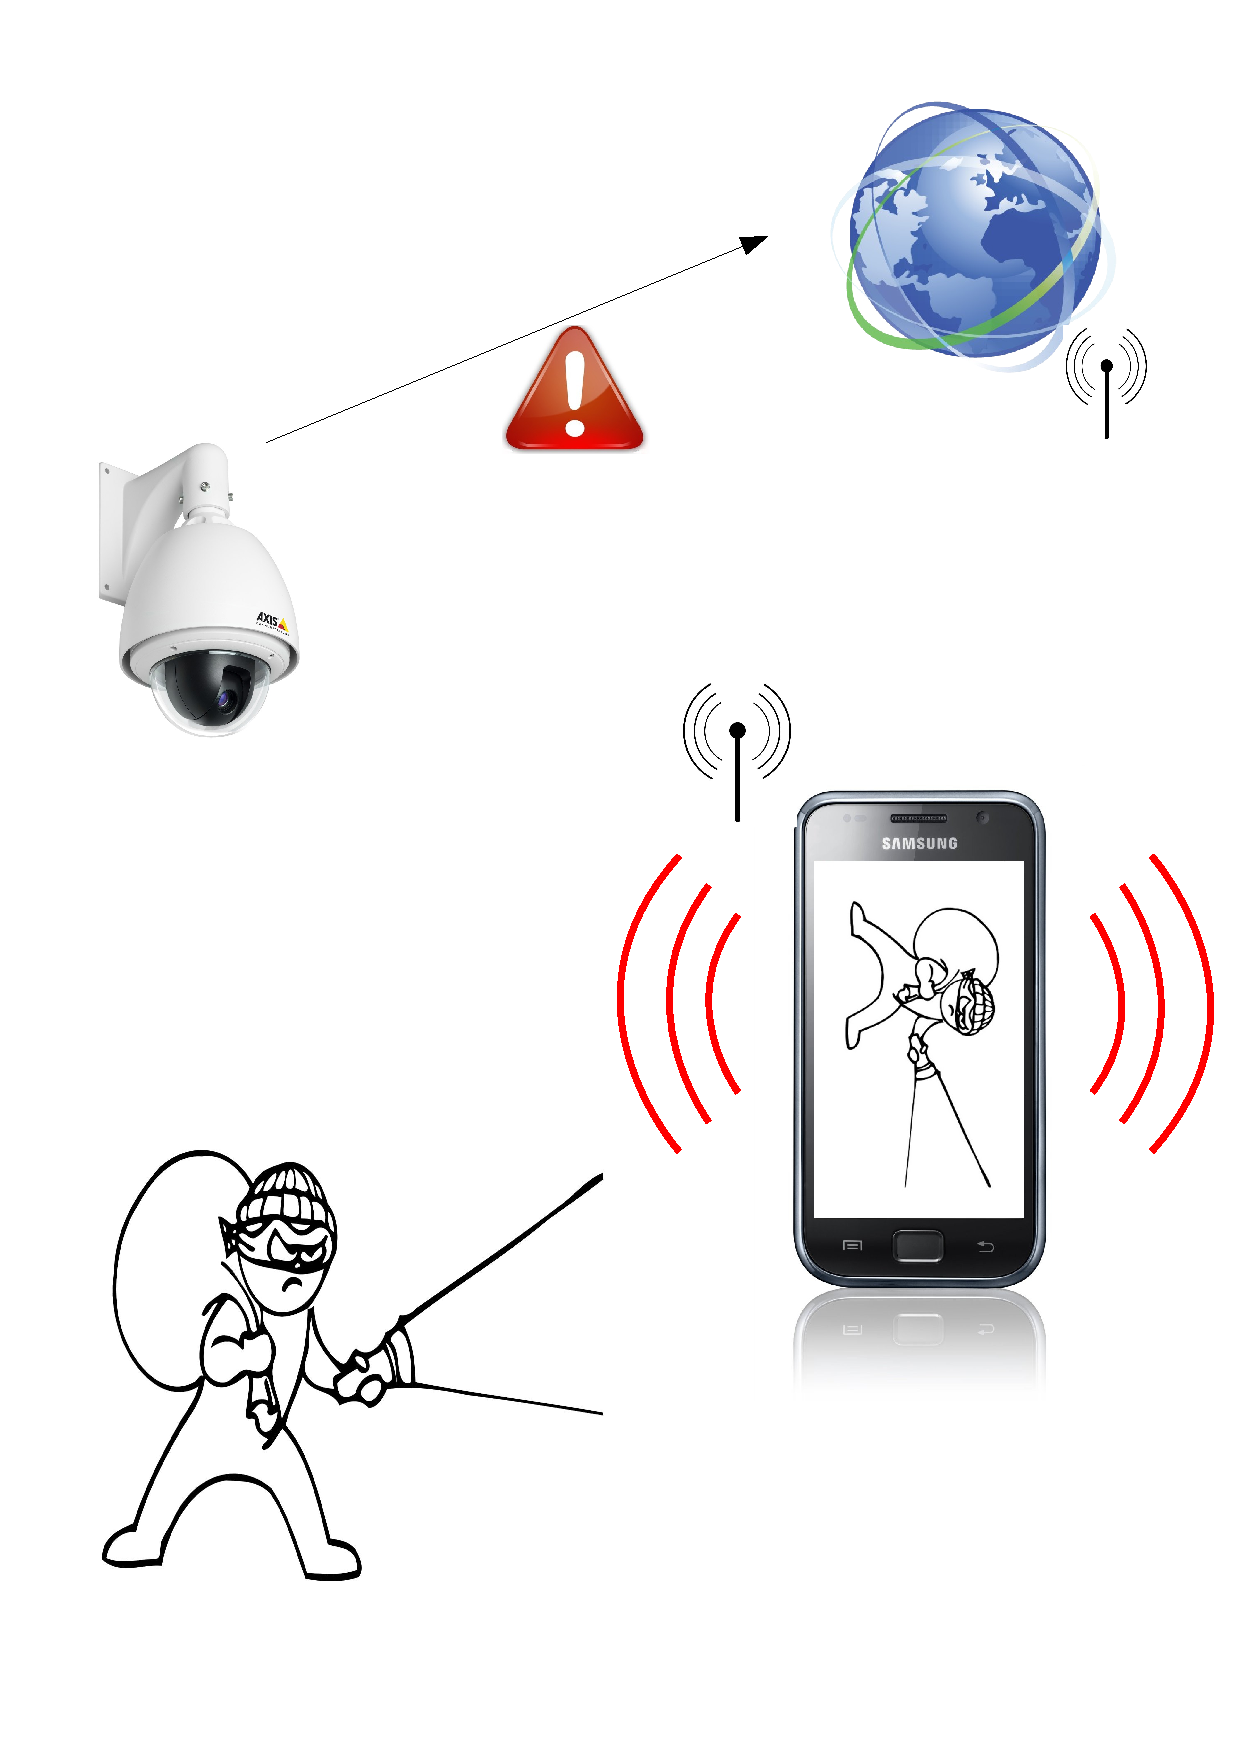
\includegraphics[scale=0.25]{Images/ImageSlide10.pdf}
\end{column}
\begin{column}{7cm}
\textbf{\textit{Caractéristiques :}} 
\begin{itemize}
    \item Réglage de la fenètre et du seuil de détection.
  	\item 1 à 10 fenètres par caméra.
  	\item Détection illimitée pour des caméras differente.
 	\item Notification via Vibration et Cliché instantanné.
 	\item Utilisation facile et intuitive.
\end{itemize}
\end{column}
\end{columns}
  \end{frame}
